\begin{quote}
\textbf{Why this appendix exists.} The body of this handbook works
through durable mechanisms --- tokens, memory floors, rooflines,
parallelism, KV arithmetic --- that do not change. But the industry
moves, and the whole point of an architecture handbook is to stay
current. In 2026 the four frontier open-weight MoE families ---
DeepSeek-V4, Kimi K3, Qwen3.8-Flash-Next, and GLM-5.3-Flash --- all
shipped within a short window. Reading them together is not a product
tour; it is a single, coherent signal about where the mechanisms in this
book are heading. Every mechanism below maps back to a chapter and an
architectural decision. Where a vendor number appears, it is tagged
{[}1P{]} (first-party) and, per this book's discipline, flagged as a
vendor-reported figure an architect should verify on their own hardware
before trusting it for their workload.
\end{quote}

\section{The Signal in One Paragraph}\label{the-signal-in-one-paragraph}

Four independent labs converged on a \textbf{second-order architectural
pattern} in 2026 --- but we should be precise about \emph{what kind} of
gain each lever delivers. The common error is to read architecture
innovation as raw capability. It is mostly \textbf{efficiency} (more
context, less cost per token) that comes out of the attention and MoE
changes below, not intelligence. The capability story --- reasoning,
post-training, test-time compute --- lives elsewhere (§6), and carries
at least as much of the frontier's real progress. We separate the two
explicitly.

\begin{figure}
\centering
\pandocbounded{\includegraphics[keepaspectratio,alt={Fig A.1 --- 2026 frontier MoE extreme sparsity: four open models, total vs activated parameters, and active fraction in single digits {[}1P{]}},width=\maxwidth{\textwidth},keepaspectratio]{figures/fig-27-2701.pdf}}
\caption{Fig A.1 --- 2026 frontier MoE extreme sparsity: four open
models, total vs activated parameters, and active fraction in single
digits {[}1P{]}}
\end{figure}

\emph{Fig A.1 --- Frontier MoE sparsity in 2026. Kimi K3 is the extreme
case: 2.8 T total / 104 B active (\textasciitilde3.7\% active);
DeepSeek-V4-Flash 284 B/13 B (\textasciitilde4.6\%); GLM-5.3-Flash 320
B/18 B (\textasciitilde5.6\%); Qwen3.8-Flash-Next 125 B/6 B
(\textasciitilde4.8\%). Active-parameter fraction in every frontier
model is now single digits --- the anchor for the Ch10
expert-parallelism serving calculus. {[}1P: arXiv 2606.19348; arXiv
2607.24653; HF Qwen/Qwen3.8-Flash-Next; HF zai-org/GLM-5.3-Flash{]}}

Three \textbf{efficiency levers} every 2026 frontier family pulled:

\begin{enumerate}
\def\labelenumi{\arabic{enumi}.}
\tightlist
\item
  \textbf{Hybrid attention as the new KV lever --- an efficiency lever,
  not (by itself) a capability lever.} Every frontier model
  re-engineered attention to shrink long-context cost at the mechanism
  level --- compressed/sparse hybrids (DeepSeek CSA+HCA), delta+sparse
  (Qwen Gated DeltaNet + QSA), delta/residual (Kimi KDA + AttnRes),
  sparse+linear (GLM). KV cache is no longer a fixed per-token constant
  we only quantize; it is a design surface the model vendor already
  optimized. The benefit is \emph{same intelligence, much
  cheaper/bigger-context inference} --- indispensable, but it does not
  by itself make the model smarter. Capability gains come from the
  post-training/reasoning stack in §6.
\item
  \textbf{MoE sparsity went extreme --- the capacity-per-FLOP lever.}
  Active-parameter fractions fell to single digits (Kimi 104B of 2.8T;
  Qwen 6B of 125B). MoE is arguably a \emph{larger} architectural
  innovation than attention: it lets a lab grow knowledge/capacity
  without proportionally growing FLOPs per token. That is why the 2026
  open landscape is heavily MoE-oriented. Expert parallelism and fused
  cross-expert communication moved from a footnote to a serving-critical
  capability.
\item
  \textbf{Efficiency is a first-class result, not an afterthought.}
  Training-stable optimizers (Muon) and post-training RL (GRPO, async
  RL) are now reported as core architecture, not tooling.
\end{enumerate}

These three form the \emph{cost/context} ledger of the frontier. The
\emph{capability} ledger --- reasoning, post-training, test-time
compute, agent harness --- is where most of the qualitative improvement
actually lives (§6). Distinguishing efficiency levers from capability
levers is the architect's first move when reading any new model card.

\section{How to read this appendix: Observed, Interpretation,
Hypothesis}\label{how-to-read-this-appendix-observed-interpretation-hypothesis}

This appendix surveys vendor-reported material, so we are careful to
separate three layers of statement that are easy to blur --- especially
in a fast-moving field full of first/``most-efficient''/3T-class claims:

\begin{itemize}
\tightlist
\item
  \textbf{Observed} --- what the vendor's technical report or model card
  actually states (e.g., ``DeepSeek-V4 reports a reduced KV
  footprint''). This is {[}1P{]} \emph{fact about the claim}, not the
  same as the third layer.
\item
  \textbf{Interpretation} --- our read of what architectural mechanism
  the report demonstrates (e.g., ``the KV reduction suggests the model
  changes how attention stores state''). This is analysis, ours, and
  could be wrong.
\item
  \textbf{Hypothesis} --- a prediction about consequence we draw for
  serving architecture (e.g., ``we expect long-context serving to become
  more memory-comfortable at equal context''). This is a testable
  {[}HYPOTHESIS{]}, not a fact.
\end{itemize}

When we write ``Four independent labs converged'' or ``MoE is arguably a
larger architectural innovation,'' read those as \textbf{Interpretation
/ Hypothesis} --- defensible reads of the frontier signal, not
independent measurements. Vendor numbers stay tagged {[}1P{]} and
flagged verify-on-own-hardware; our reads sit one register lower and
should be read with the same skepticism we ask of any vendor claim. The
practical rule: \emph{if it's a percentage from a report, it's Observed
{[}1P{]}; if it's a claim about what the industry trend means, it's ours
--- treat it as analysis, tune it against the reader's real workload.}

\section{DeepSeek-V4 --- Making Long Context Cheap by Re-Architecting
Attention}\label{deepseek-v4-making-long-context-cheap-by-re-architecting-attention}

\textbf{Decisive fact {[}1P: arXiv 2606.19348; HF
deepseek-ai/DeepSeek-V4-Pro{]}:} V4-Pro is 1.6 T total / 49 B activated,
V4-Flash 284 B / 13 B activated, both 1M-token context, MIT-licensed.
Its hybrid attention combines Compressed Sparse Attention (CSA) and
Heavily Compressed Attention (HCA). At 1M context, DeepSeek reports
\textbf{\textasciitilde27\% (Pro) / \textasciitilde10\% (Flash) of
V3.2's single-token inference FLOPs and \textasciitilde10\% /
\textasciitilde7\% of its KV cache}.

\textbf{What this means for the architect (ties to Ch7 Memory, Ch8
Compute).} This is the sharpest confirmation yet that \emph{KV-per-token
is a moving target}. \hyperref[chap:7]{Chapter 7}'s arithmetic (per-token × context) is a
floor for a given architecture; DeepSeek shows the \emph{constant factor
itself} can be cut \textasciitilde10× without changing the model's
parameter count. The architectural decision shifts from ``how much KV
memory does this context need?'' to ``which KV scheme does this model
use, and is its vendor-published saving reproducible on my serving
stack?''

\section{Kimi K3 --- The First Open 3T-Class Model, and the MoE-Sparsity
Extreme}\label{kimi-k3-the-first-open-3t-class-model-and-the-moe-sparsity-extreme}

\textbf{Decisive fact {[}1P: arXiv 2607.24653; HF
moonshotai/Kimi-K3{]}:} 2.8 T total / 104 B activated, native vision, 1M
context. Built on \textbf{Kimi Delta Attention (KDA)} +
\textbf{Attention Residuals (AttnRes)}, with \textbf{Stable LatentMoE}
activating just \textbf{16 of 896 routed experts} per token. Claims
\textasciitilde{}\textbf{2.5× scaling efficiency} over Kimi K2. Weights
are QAT-trained from SFT onward with \textbf{MXFP4 weights / MXFP8
activations}. Full weights are released --- the first open 3T-class
model.

\textbf{What this means for the architect (ties to Ch3 Model, Ch10
Parallelism).} A model whose \emph{total} size is 2.8 T but whose
\emph{activated} footprint is 104 B is the ultimate demonstration of
Ch3's total-vs-activated distinction and Ch10's expert-parallelism
doctrine. Serving it is not ``2.8 T is too big to fit'' --- it is ``fit
and feed 104 B active, plus the KV for our context, while sharding and
scheduling the expert fabric.'' The decision surface is expert-parallel
communication and fused cross-expert kernels, not raw capacity.

\section{Qwen3.8-Flash-Next --- The Qwen4 Architecture Preview,
Prioritizing
Cost-Performance}\label{qwen3.8-flash-next-the-qwen4-architecture-preview-prioritizing-cost-performance}

\textbf{Decisive fact {[}1P: HF Qwen/Qwen3.8-Flash-Next; GitHub
QwenLM/Qwen3.8-Flash-Next{]}:} 125 B total / 6 B activated, plus a
separate 51 B of \textbf{N-gram embedding} parameters (offloadable to
host memory). Native 262 K context (YaRN to 1M). \textbf{Hybrid
attention: Gated DeltaNet (GDN) + Qwen Sparse Attention (QSA)}, where
QSA operates at the \emph{micro-block} level; \textbf{Gated Residual}
widens the residual stream; 512 MoE experts (10 routed + 1 shared per
token); Muon + AdamW. Reported training cost \textasciitilde1/9 of
Qwen3.7-Plus.

\textbf{What this means for the architect (ties to Ch3, Ch5 Model
Selection, Ch16 TCO).} Qwen's N-gram embedding split is the most
architecturally novel item: it shows that \emph{parameter scaling and
compute scaling can be decoupled} --- a large embedding table can trade
host-RAM bandwidth for on-GPU capacity when the compute budget is the
binding constraint. This refines the model-selection calculus in Ch5: an
architect comparing candidates now weighs not just total/active params
but heterogeneous memory (on-GPU weights vs offloadable embeddings) and
its serving overlap.

\section{GLM-5.3-Flash --- First Natively Multimodal GLM,
Efficiency-Branded}\label{glm-5.3-flash-first-natively-multimodal-glm-efficiency-branded}

\textbf{Decisive fact {[}1P: HF zai-org/GLM-5.3-Flash; arXiv
2602.15763{]}:} 320 B total / 18 B activated, 1M native context, 131 K
output. First natively multimodal model in the GLM-5 series
(text/image/video). Hybrid \textbf{sparse+linear attention} (first in
the series) with \textasciitilde3× attention-compute and
\textasciitilde4.4× KV-cache reductions; Manifold-Constrained
Hyper-Connections (mHC); W8A8 quantization with mixed-cache
(INT8/FP8/BF16); Encode-Prefill-Decode serving. MIT weights. Z.ai
positions it as approaching Claude Opus 4.8 on coding/agentic at
\textasciitilde1/10 the price.

\textbf{What this means for the architect (ties to Ch7 Memory, Ch8
Compute, Ch19 Agentic).} GLM's coupling of hybrid attention with
\emph{native multimodality} shows the model border is remaking: ``LLM''
and ``vision/audio model'' are converging in a single weight set, which
changes workload characterization (Ch4) --- a multimodal prompt has a
different token/KV profile than text-only. And mHC + attention-mixing
being reported as \emph{scaling-efficiency} results reinforces Ch8's
point that compute arithmetic is architecture-specific, not universal.

\section{What This Means for the Handbook's Canonical
Arithmetic}\label{what-this-means-for-the-handbooks-canonical-arithmetic}

\begin{figure}
\centering
\pandocbounded{\includegraphics[keepaspectratio,alt={Fig A.2 --- The KV constant and FLOP/token are a moving target: hybrid attention cuts both at the mechanism. Canonical 70B dense full-MHA = 100\%; DeepSeek-V4-Flash ≈ 7\% KV / 10\% FLOP, V4-Pro ≈ 10\% / 27\%, GLM-5.3-Flash ≈ 23\% KV / \textasciitilde33\% attention-compute {[}DERIVED from 1P claims: arXiv 2606.19348; HF zai-org{]}},width=\maxwidth{\textwidth},keepaspectratio]{figures/fig-27-2704.pdf}}
\caption{Fig A.2 --- The KV constant and FLOP/token are a moving target:
hybrid attention cuts both at the mechanism. Canonical 70B dense
full-MHA = 100\%; DeepSeek-V4-Flash ≈ 7\% KV / 10\% FLOP, V4-Pro ≈ 10\%
/ 27\%, GLM-5.3-Flash ≈ 23\% KV / \textasciitilde33\% attention-compute
{[}DERIVED from 1P claims: arXiv 2606.19348; HF zai-org{]}}
\end{figure}

\emph{Fig A.2 --- Same message as \hyperref[fig:7.1]{Fig 7.1}'s GQA line, taken to the
frontier: the per-token KV and FLOP ``constants'' of \hyperref[chap:7]{Chapter 7}/8 are not
universal --- they are LLaMA-style floors that hybrid attention
re-architects down at the mechanism. Percentages are each model's gain
over its own predecessor (e.g.~V3.2→V4, GLM-5.x steps), shown against
the canonical 70B dense full-MHA reference so the floors stay
comparable. An architect who re-derives them per candidate model avoids
both over- (sizing a 7\% KV model as if it were 100\%) and
under-provisioning. Values are vendor-published {[}1P{]}, not yet
independently reprofiled on a serving stack (see §5).}

The book's canonical scenario is a 70B dense FP16,
\textasciitilde9.2K-token RAG workload on 8×H100. The 2026 frontier does
not invalidate it --- it \emph{refines} the interpretation an architect
should carry:

\begin{itemize}
\tightlist
\item
  The \textbf{KV constant} (Ch7: \textasciitilde2.5 MB/token FP16,
  \textasciitilde1.3 MB 8-bit) is a LLaMA-style floor. Hybrid-attention
  models cut it 4--10× at the mechanism, so ``context fits on N GPUs''
  must be re-derived per model, not looked up once. {[}1P{]}
\item
  The \textbf{roofline} (Ch8) still holds; what changed is where a
  frontier model's prefill/decode ride it. Vendor-reported FLOP/KV
  reductions are {[}1P{]} but not yet independently reprofiled --- an
  architect should re-run Ch8's measurement on the candidate model
  before betting capacity. {[}1P{]} → {[}VERIFY-candidate{]}
\item
  The \textbf{MoE memory decision} (Ch10) is now dominated by active
  parameters + KV + expert-fabric comm, not total size. {[}1P{]}
\end{itemize}

None of this changes the book's \emph{mechanisms}; it changes the
\emph{constants} an architect plugs into them. This is exactly why we
wrote the arithmetic as verifiable, first-principles reasoning rather
than as a fixed catalog of numbers.

\section{Where 2026 Capability Actually Comes From (beyond
Architecture)}\label{where-2026-capability-actually-comes-from-beyond-architecture}

A recurring error --- easy to fall into after reading four new model
cards --- is to attribute frontier gains to the attention mechanism
splashed across the front page. The industry is converging not just on
\emph{architectures} (MoE + efficient attention + very long context) but
on a \emph{multi-layered recipe} in which architecture is one
ingredient, and arguably not the dominant one. A qualitative
decomposition {[}VERIFY: qualitative, not a measured percentage{]}:

\begin{longtable}[]{@{}
  >{\raggedright\arraybackslash}p{0.5000\linewidth}
  >{\raggedright\arraybackslash}p{0.5000\linewidth}@{}}
\toprule\noalign{}
\begin{minipage}[b]{\linewidth}\raggedright
Lever
\end{minipage} & \begin{minipage}[b]{\linewidth}\raggedright
Primary effect
\end{minipage} \\
\midrule\noalign{}
\endhead
\bottomrule\noalign{}
\endlastfoot
Post-training / RL / reasoning & Capability (the largest single source
today) \\
Test-time compute & Capability on hard tasks (more compute on hard
problems) \\
Training data + optimization & General capability \\
MoE / parameter scaling & Capacity per FLOP \\
Attention innovation & Context + efficiency (makes the above
affordable) \\
Inference / runtime optimization & Cost + latency \\
Agent harness / tool use & Real-world task completion \\
Multimodal architecture & New modalities \\

\label{tab:27.1}\end{longtable}

\textbf{The most underestimated layer is the one the model card almost
never shows: post-training.} Two models with broadly similar
architectures and pre-training can end up materially different when one
went through mediocre post-training and the other excellent. The recipe
--- the same families every lab now runs --- is what carries much of the
qualitative gap:

\begin{itemize}
\tightlist
\item
  RLVR / reinforcement learning for reasoning
\item
  synthetic reasoning data
\item
  verifier-based training
\item
  preference optimization
\item
  curriculum learning
\item
  tool-use training and agent trajectories
\item
  coding-specific trajectories
\item
  multimodal reasoning
\item
  long-horizon interaction training
\end{itemize}

This is why architecture alone never tells an architect how good a
frontier model is, and why the decision can no longer stop at ``which
model'' --- the marginal capability may live in the post-training and
the runtime that wraps it.

\begin{figure}
\centering
\pandocbounded{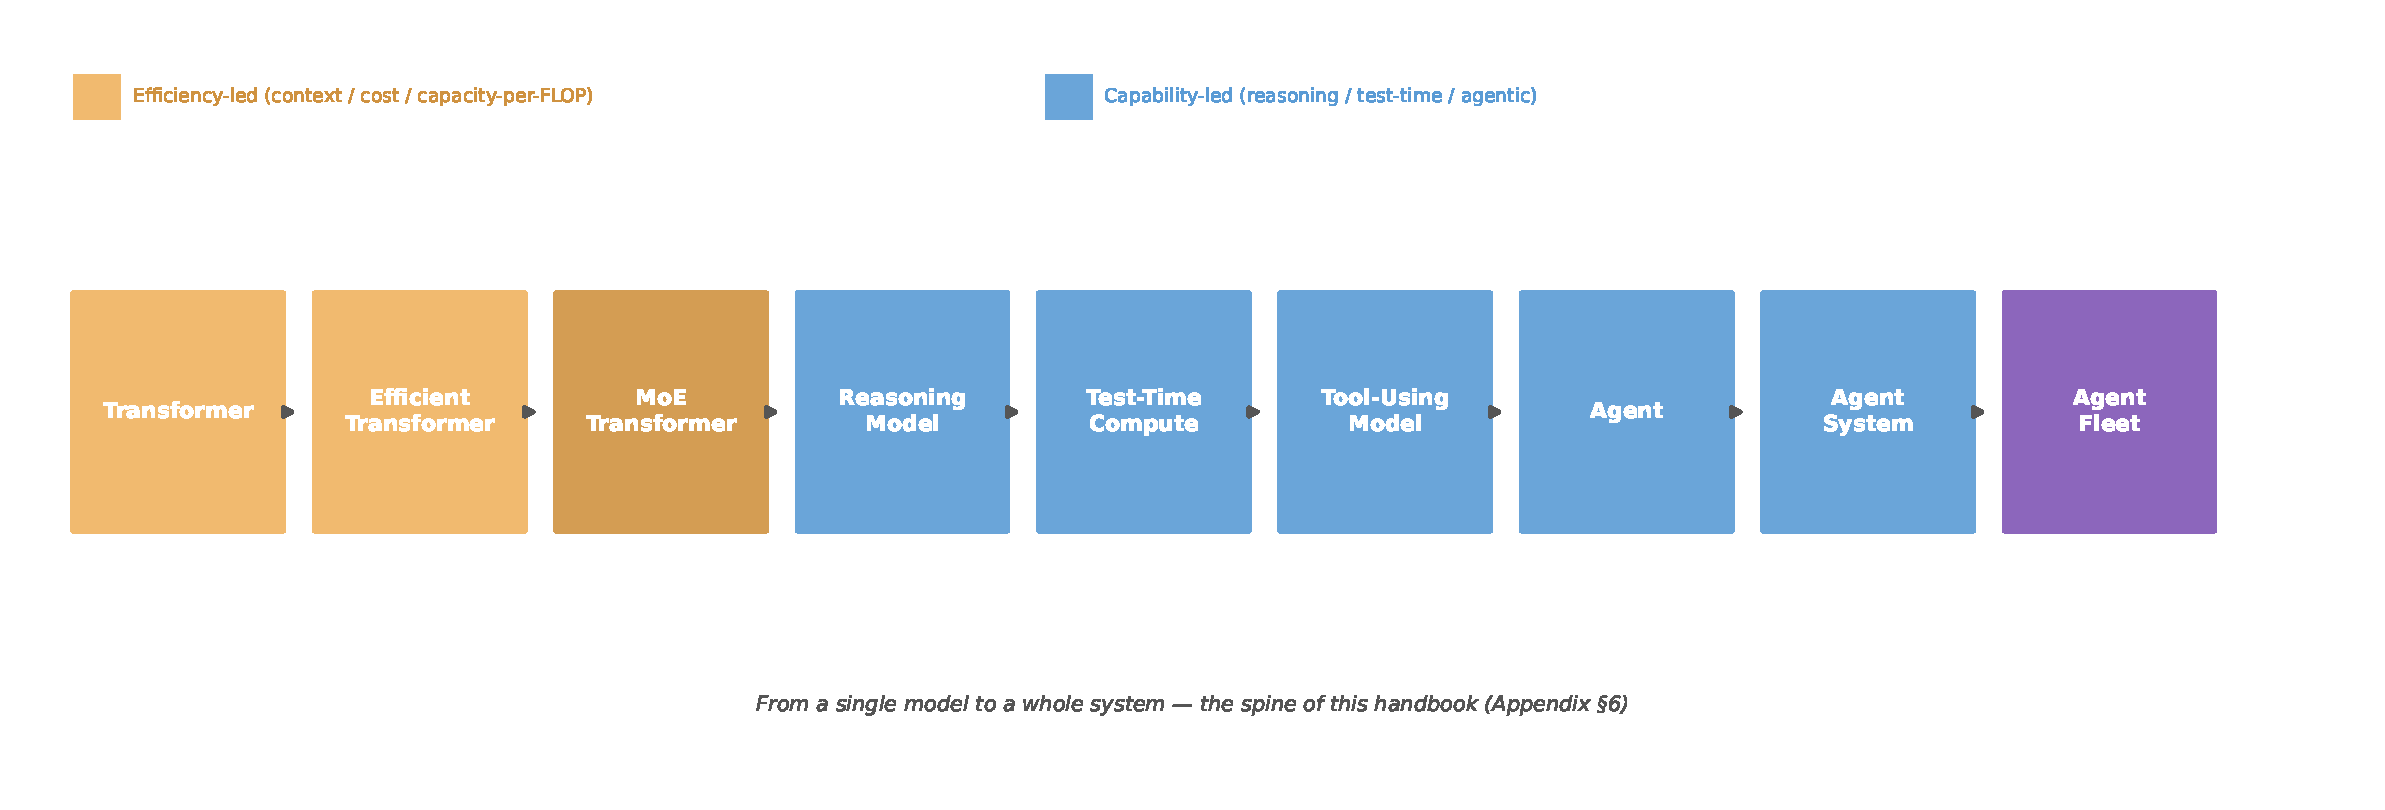
\includegraphics[keepaspectratio,alt={Fig A.3 --- The layered evolution of frontier systems, colour-coded by efficiency-led (amber) vs capability-led (blue) stages, from a single Transformer to the whole fleet (Appendix §6)},width=\maxwidth{\textwidth},keepaspectratio]{figures/fig-27-2703.pdf}}
\caption{Fig A.3 --- The layered evolution of frontier systems,
colour-coded by efficiency-led (amber) vs capability-led (blue) stages,
from a single Transformer to the whole fleet (Appendix §6)}
\end{figure}

\emph{Fig A.3 --- From a single model to a whole system. The earlier
stages (Transformer, Efficient, MoE) are largely }efficiency-led* ---
they make inference affordable and raise capacity-per-FLOP. The later
stages (Reasoning, Test-Time Compute, Tool-Using, Agent, Agent System,
Agent Fleet) are \emph{capability-led} --- they raise effective
intelligence. This chain is the spine of the handbook: tokens (Ch1--9),
parallelism (Ch10), serving (Ch11--16), fleet \& agents (Ch17--26).
{[}INTERPRETATION --- synthesis of the chapters' arithmetic, not a
single measurement{]}*

This chain is the spine of this handbook --- from a single model's
tokens (Ch1--9) to parallelism (Ch10), serving (Ch11--16), and finally
the fleet of specialised models and agents (Ch17--26). It also explains
why two models with broadly similar base architectures can have very
different practical intelligence (post-training/reasoning), and why an
agent runtime can lift real-world performance without changing model
weights at all: \textbf{model intelligence ≠ system intelligence
anymore.}

\section{The Frontier Question: Where Should Intelligence
Live?}\label{the-frontier-question-where-should-intelligence-live}

The most useful lens for an AI Solution Architect in 2026 is not ``which
attention mechanism does the model card list?'' but \emph{where the
intelligence and the compute budget should be placed}:

\begin{figure}
\centering
\pandocbounded{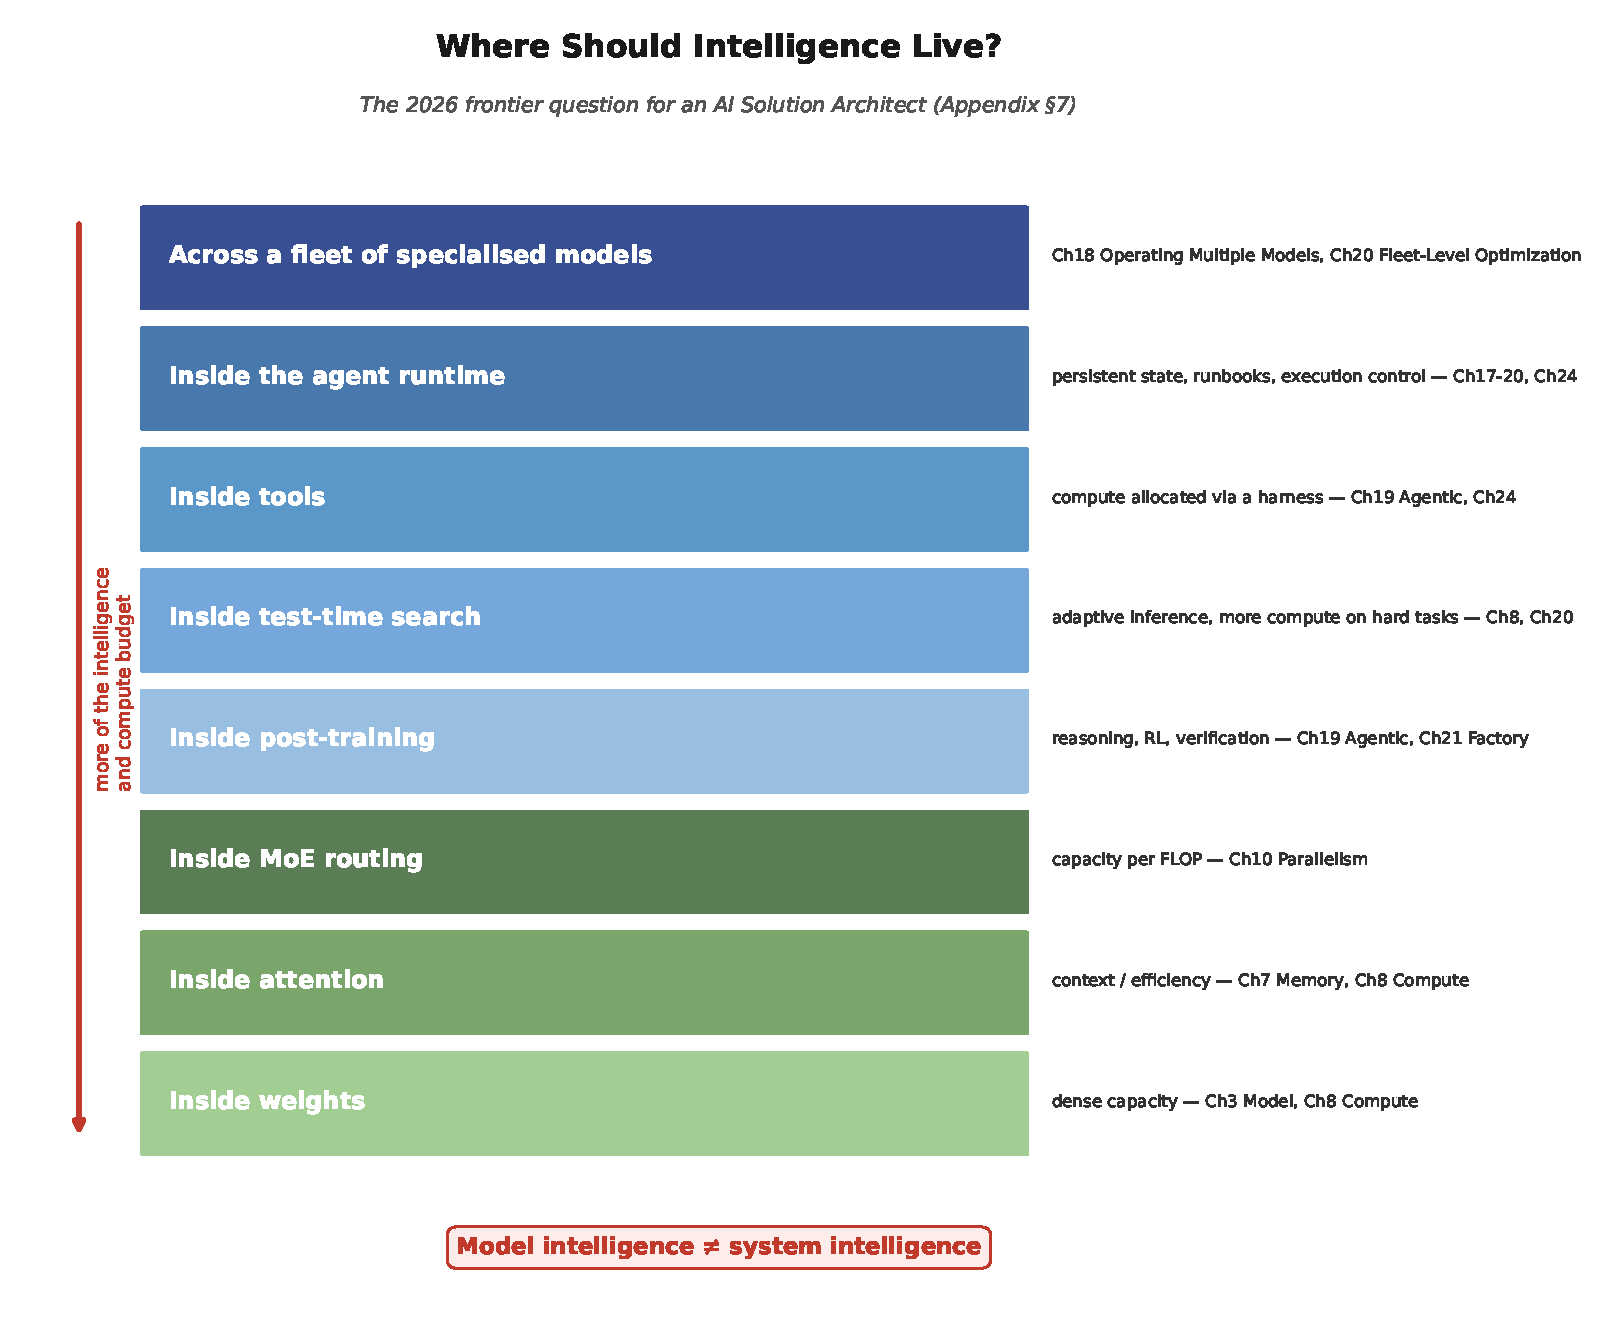
\includegraphics[keepaspectratio,alt={Fig A.4 --- Where should intelligence live? Eight host layers, from inside the weights up to across a fleet of specialised models, each mapped to the chapters of this handbook that give the tooling to evaluate it (Appendix §7)},width=\maxwidth{\textwidth},keepaspectratio]{figures/fig-27-2702.pdf}}
\caption{Fig A.4 --- Where should intelligence live? Eight host layers,
from inside the weights up to across a fleet of specialised models, each
mapped to the chapters of this handbook that give the tooling to
evaluate it (Appendix §7)}
\end{figure}

\emph{Fig A.4 --- The placement ladder. Every host layer that can carry
intelligence is a place the architect may choose to push capability or
cost; this book gives the arithmetic and decision framework for each
(Ch3/7/8 weights \& attention, Ch10 MoE routing, Ch19/21 post-training,
Ch8/20 test-time, Ch19/24 tools, Ch17--20 runtime, Ch18/20 fleet).
{[}INTERPRETATION/ILLUSTRATIVE per Appendix A's three-layer rule{]}}

Every host layer maps to chapters in this book:

\begin{itemize}
\tightlist
\item
  \textbf{Inside weights} (dense capacity) --- Ch3 Model, Ch8 Compute
\item
  \textbf{Inside attention} (context / efficiency) --- Ch7 Memory, Ch8
  Compute
\item
  \textbf{Inside MoE routing} (capacity per FLOP) --- Ch10 Parallelism
\item
  \textbf{Inside post-training} (reasoning, RL, verification) --- Ch19
  Agentic, Ch21 AI Factory
\item
  \textbf{Inside test-time search} (adaptive inference, more compute on
  hard tasks) --- Ch8 Compute, Ch20 Fleet-Level Optimization
\item
  \textbf{Inside tools} (compute allocated via a harness) --- Ch19
  Agentic, Ch24 Red/Green Team
\item
  \textbf{Inside the agent runtime} (persistent state, runbooks,
  execution control) --- Ch17--20, Ch24
\item
  \textbf{Across a fleet of specialised models} --- Ch18 Operating
  Multiple Models, Ch20 Fleet-Level Optimization
\end{itemize}

Deciding where intelligence lives --- rather than which attention
variant a model card lists --- is the actual job of an AI Solution
Architect. The frontier of 2026 makes that explicit: DeepSeek-V4-Flash
vs Qwen3.8-Flash vs a fleet of specialised agents on a 2×DGX cluster are
no longer merely \emph{model} choices; they are
\emph{placement-of-intelligence} choices whose economics this handbook's
chapters give the tools to evaluate.

\section{One-Hand Sources (all {[}1P{]})}\label{one-hand-sources-all-1p}

\begin{itemize}
\tightlist
\item
  DeepSeek-V4: technical report arXiv:2606.19348; model card
  https://huggingface.co/deepseek-ai/DeepSeek-V4-Pro; org
  https://github.com/deepseek-ai
\item
  Kimi K3: technical report arXiv:2607.24653; model card
  https://huggingface.co/moonshotai/Kimi-K3;
  https://github.com/moonshotai
\item
  Qwen3.8-Flash-Next: technical report
  https://github.com/QwenLM/Qwen3.8-Flash-Next/blob/main/tech\_report.pdf;
  model card https://huggingface.co/Qwen/Qwen3.8-Flash-Next
\item
  GLM-5.3-Flash: technical report arXiv:2602.15763; model card
  https://huggingface.co/zai-org/GLM-5.3-Flash;
  https://github.com/zai-org/GLM-5
\end{itemize}

\emph{Compiled 2026-08-30 from the models' official technical reports
and first-party model cards; all parameters/claims are vendor-reported
{[}1P{]} and per this handbook's discipline carry a
verify-on-own-hardware caveat.}
